\documentclass[a4paper,12pt]{article}
\usepackage[utf8]{inputenc}
\usepackage{graphicx}
\usepackage{fancyhdr}
\usepackage{amsmath}
\usepackage{adjustbox}
\usepackage{mathtools}
\usepackage{float}
\usepackage[spanish, es-nodecimaldot]{babel} 
\usepackage{lastpage}
\usepackage{amssymb} % Para símbolos matemáticos adicionales
\usepackage{hyperref}
\usepackage{cleveref}
%\usepackage[none]{hyphenat}
\usepackage{array}

\usepackage{multirow}
\usepackage{textcomp}
\usepackage[left=2.5cm, right=2.5cm, top=3cm, bottom=3cm]{geometry}

\graphicspath{{Imagenes/}}

% Encabezado y pie de página
\pagestyle{fancy}
\fancyhf{}
\setlength{\headheight}{30 pt}
\renewcommand{\headrulewidth}{0.2pt}
\fancyhead[R]{\begin{tabular}{@{}l@{}}
\includegraphics[scale=0.4]{escudo.PNG}\end{tabular}}
\fancyhead[L]{\begin{tabular}{@{}c@{}} \textbf{Robótica I - Año: 2024} \\ Trabajo Práctico 4: Cinemática Directa \end{tabular}}


\fancyfoot[R]{\thepage}
\fancyfoot[C]{\begin{tabular}{@{}c@{}}\textbf{BORQUEZ PEREZ Juan Manuel}\\ \textbf{Legajo 13567}\end{tabular}}
\renewcommand{\footrulewidth}{0.2pt}

\begin{document}

\begin{titlepage}
    \centering
    \vspace*{5cm}
    {\Huge\bfseries Informe de Trabajo Práctico N°4}\\
    \vspace{0.2cm}
    {\Large \textbf{Cinemática Directa}}\\
    \vspace{0.5cm}
    {\Large Robótica I}\\
    \vspace{0.5 cm}
    {\Large Ingeniería en Mecatrónica}\\
    \vspace{0.2 cm}
    {\Large Facultad de Ingeniería - UNCUYO}\\
    \vspace{1.5cm}
    Alumno: Juan Manuel BORQUEZ PEREZ\\
    Legajo: 13567\\
    \vfill
    {\begin{tabular}{@{}c@{}}
\includegraphics[scale=0.4]{escudo.PNG}\end{tabular}}\hspace{10pt}
    %Año 2023
\end{titlepage}

\section{Ejercicio 1.}
\textbf{Trabaje en Matlab y resuelva la cinemática directa del Paint Mate 200iA (FANUC), para los siguientes arreglos de variables articulares}

\begin{figure}[H]
    \centering
    \begin{adjustbox}{scale = 0.35, max width=\columnwidth}
        \framebox{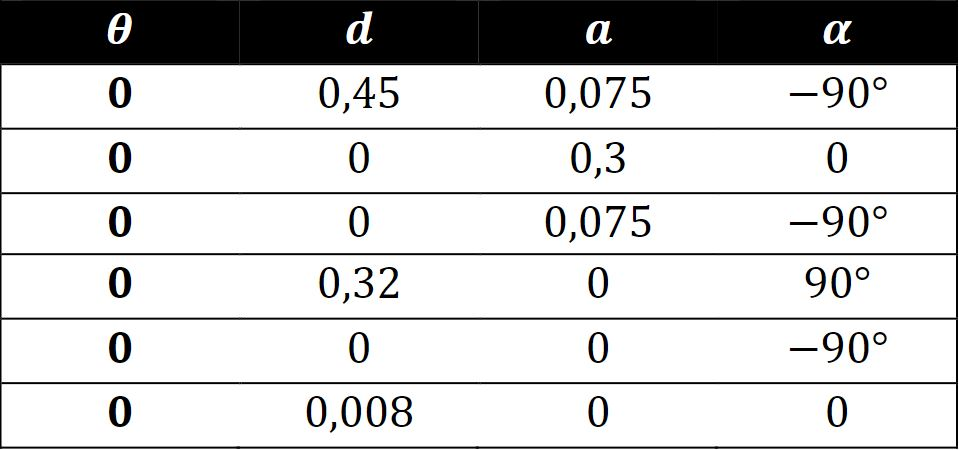
\includegraphics{1-DH_fanuc.JPG}}
    \end{adjustbox}
    \caption{Parametros DH Fanuc.}
\end{figure}

\subsection{}
Coordenadas articulares:
\begin{equation*}
    \overline{q}_1 = 
    \begin{bmatrix}
        0\,;0\,;0\,;0\,;0\,;0
    \end{bmatrix}
\end{equation*}

Matriz de transformación total:
\[\left(\begin{array}{cccc} 1.0 & 0 & 0 & 0.45\\ 0 & -1.0 & 0 & 0\\ 0 & 0 & -1.0 & 0.122\\ 0 & 0 & 0 & 1.0 \end{array}\right)\]

\subsection{}
Coordenadas articulares:
\begin{equation*}
    \overline{q}_2 = 
    \begin{bmatrix}
        \pi/4;-\pi/2\,\;0\,;0\,;0\,;0
    \end{bmatrix}
\end{equation*}

Matriz de transformación total:
\[\left(\begin{array}{cccc} 0 & 0.7071 & 0.7071 & 0.285\\ 0 & -0.7071 & 0.7071 & 0.285\\ 1.0 & 0 & 0 & 0.825\\ 0 & 0 & 0 & 1.0 \end{array}\right)\]

\subsection{}
Coordenadas articulares:
\begin{equation*}
    \overline{q}_3 = 
    \begin{bmatrix}
        \pi/5\,;-2\pi/5\,;-\pi/10\,;\pi/2\,;3\pi/10\,;-\pi/2
    \end{bmatrix}
\end{equation*}

Matriz de transformación total:
\[\left(\begin{array}{cccc} 0 & 1.0 & 0 & 0.3946\\ 0 & 0 & 1.0 & 0.2947\\ 1.0 & 0 & 0 & 0.8103\\ 0 & 0 & 0 & 1.0 \end{array}\right)\]

\subsection{}
Coordenadas articulares:
\begin{equation*}
    \overline{q}_4 = 
    \begin{bmatrix}
        -0.61\,;-0.15\,;-0.30\,;1.40\,;1.90\,;-1.40
    \end{bmatrix}
\end{equation*}

Matriz de transformación total:
\[\left(\begin{array}{cccc} 0.8941 & 0.3322 & 0.3003 & 0.4764\\ -0.3545 & 0.1156 & 0.9279 & -0.3239\\ 0.2735 & -0.9361 & 0.2211 & 0.2411\\ 0 & 0 & 0 & 1.0 \end{array}\right)\]

\begin{figure}[H]
    \centering
    \begin{adjustbox}{max width=\columnwidth}
        \framebox{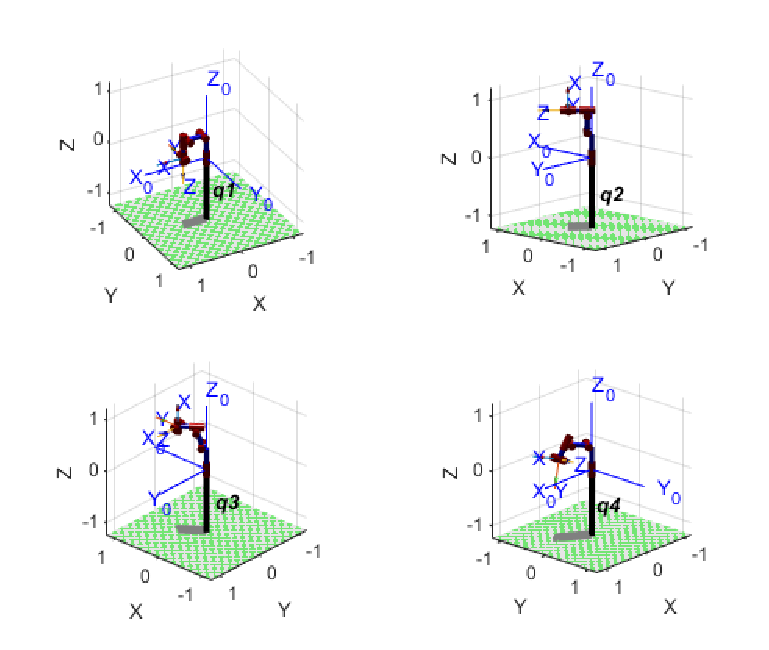
\includegraphics{2-Ejercicio_1_posiciones.pdf}}
    \end{adjustbox}
    \caption{Posiciones articulares correspondientes.}
\end{figure}

\section{Ejercicio 2.}
\subsection{Verificación del robot}
Por observación de la matriz DH dada en comparación con la propuesta
en el TP3 para el mismo tipo de robot se puede identificar que se refieren
a distintos modelos. La que se confeccionó para el TP3 corresponde al 
SCARA IRB 910SC-3/0.45 mientras que la que se indica aquí corresponde al
SCARA IRB 910SC-3/0.55. La diferencia se presenta en el parámetro $L$ (\cref{diferencia SCARA}), que se corresponde
con el parámetro $a$ del $S_1$, en la fila 1 de la matrices DH (\cref{DH TP3} y \cref{DH TP4}). Además
se puede observar en la \cref{DH TP4} que los sistemas 2 y 1 coinciden en origen a lo largo del eje z
y también el sistema 4 comparte origen en el extremo final con el sistema 3, mientras que en \cref{DH TP3}
se tomó un desplazamiento en el eje z entre el sistema 1 y 2, y también entre el sistema 3 y 4.
Luego existe una diferencia en la medida tomada para la separación entre el sistema de la base
y el sistema 1.

\begin{figure}[H]
    \centering
    \begin{adjustbox}{scale = 0.8,max width=\columnwidth}
        \framebox{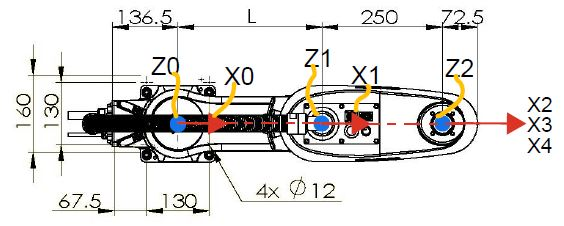
\includegraphics{3-SCARA_L.JPG}}
    \end{adjustbox}
    \caption{Indicación del parámetro L.}
    \label{diferencia SCARA}
\end{figure}

\begin{figure}[H]
    \centering
    \begin{adjustbox}{scale = 0.72, max width=\columnwidth}
        \framebox{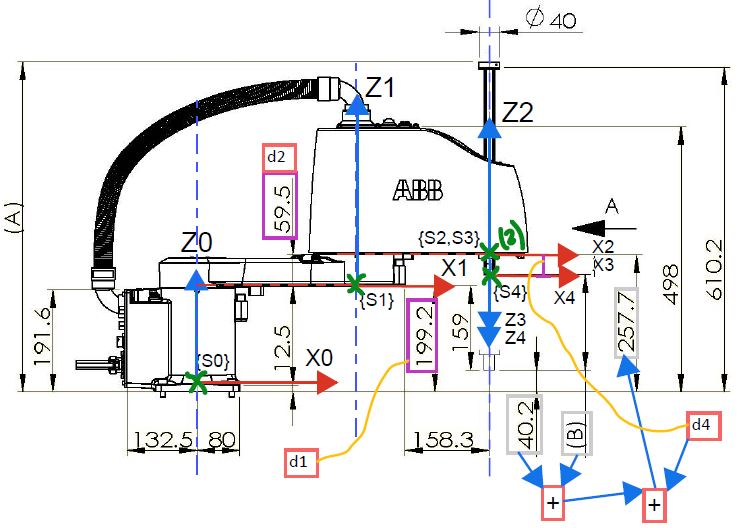
\includegraphics{4-SCARA_lateral.JPG}}
    \end{adjustbox}
    \caption{Vista lateral robot.}
    \label{vista lateral}
\end{figure}

\begin{table}[H]
    \centering
    \begin{tabular}{|c|c|c|c|c|c|}
    \hline
    Sistema & $\theta$  & $d$           & $a$      & $\alpha$ & $\sigma$ \\ \hline
    1       & $q_1$     & $0.1992$      & $0.200$  & 0.000    & 0        \\ \hline
    2       & $q_2$     & $0.0595$      & $0.250$  & 0.000    & 0        \\ \hline
    3       & $0.000$   & $q_3$         & $0.000$  & $\pi$      & 1        \\ \hline
    4       & $q_4$     & $0.0375$      & $0.000$  & 0.000    & 0        \\ \hline
    \end{tabular}
    \caption{Parámetros DH TP3.}
    \label{DH TP3}
\end{table}

\begin{table}[H]
    \centering
    \begin{tabular}{|c|c|c|c|c|c|}
    \hline
    Sistema & $\theta$  & $d$           & $a$      & $\alpha$ & $\sigma$ \\ \hline
    1       & $q_1$     & $0.195$       & $0.300$  & 0.000    & 0        \\ \hline
    2       & $q_2$     & $0.000$       & $0.250$  & 0.000    & 0        \\ \hline
    3       & $0.000$   & $q_3$         & $0.000$  & $\pi$      & 1        \\ \hline
    4       & $q_4$     & $0.000$       & $0.000$  & 0.000    & 0        \\ \hline
    \end{tabular}
    \caption{Parámetros DH TP4.}
    \label{DH TP4}
\end{table}

\begin{figure}[H]
    \centering
    \begin{adjustbox}{max width=\columnwidth}
        \framebox{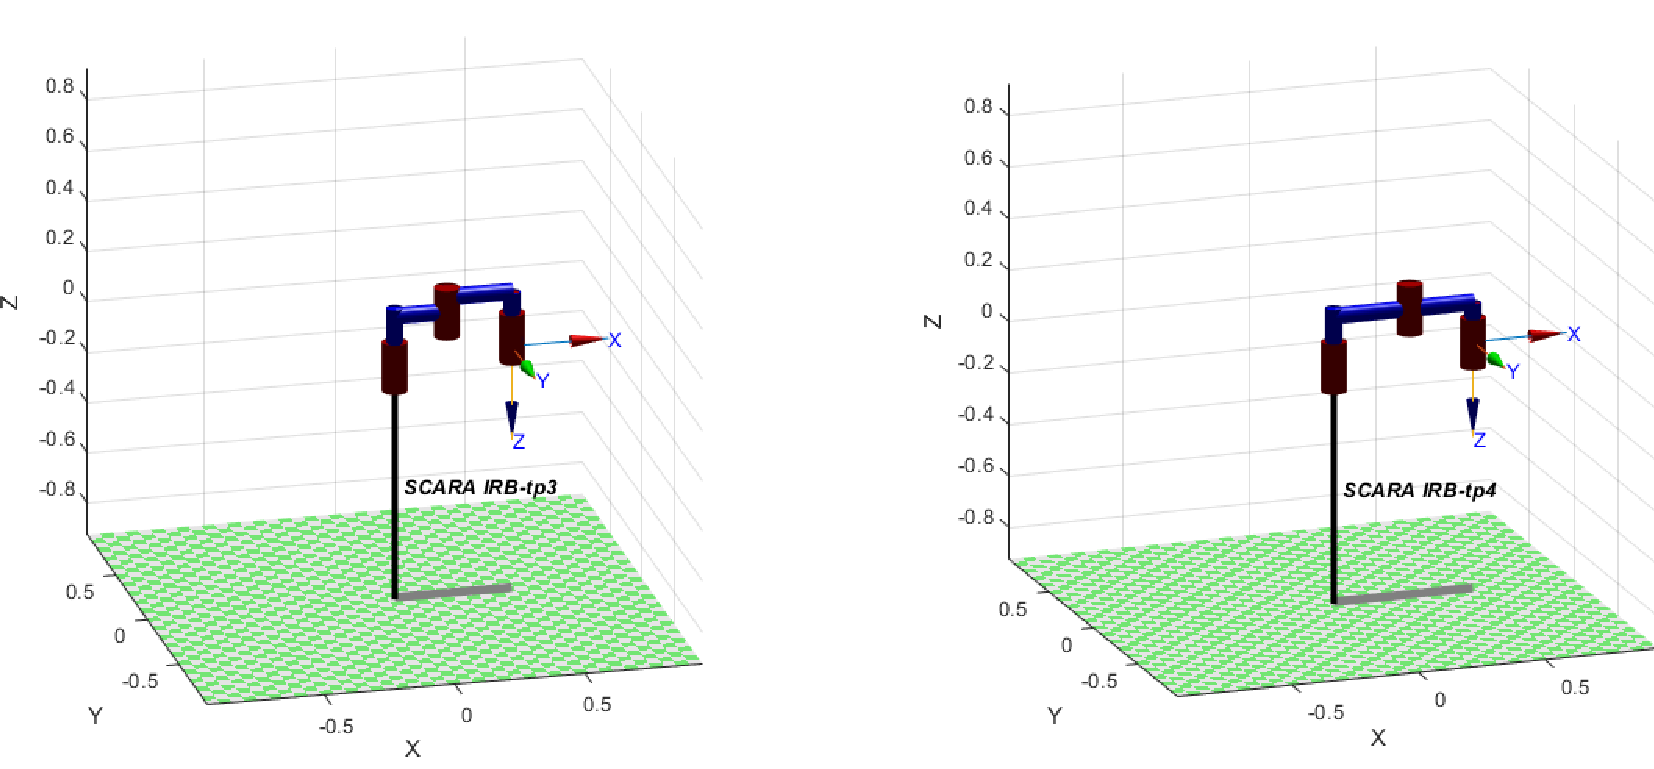
\includegraphics{4-Ejercicio_1_verificacion.pdf}}
    \end{adjustbox}
    \caption{Comparación de las definiciones.}
    \label{comparacion}
\end{figure}
En la anterior figura se comparan las definiciones. Considero que es mas eficiente la definición
dada en este TP en lugar de los desplazamientos de los sistemas como se presentó en el TP3.


\begin{figure}[H]
    \centering
    \begin{adjustbox}{scale = 0.85, max width=\columnwidth}
        \framebox{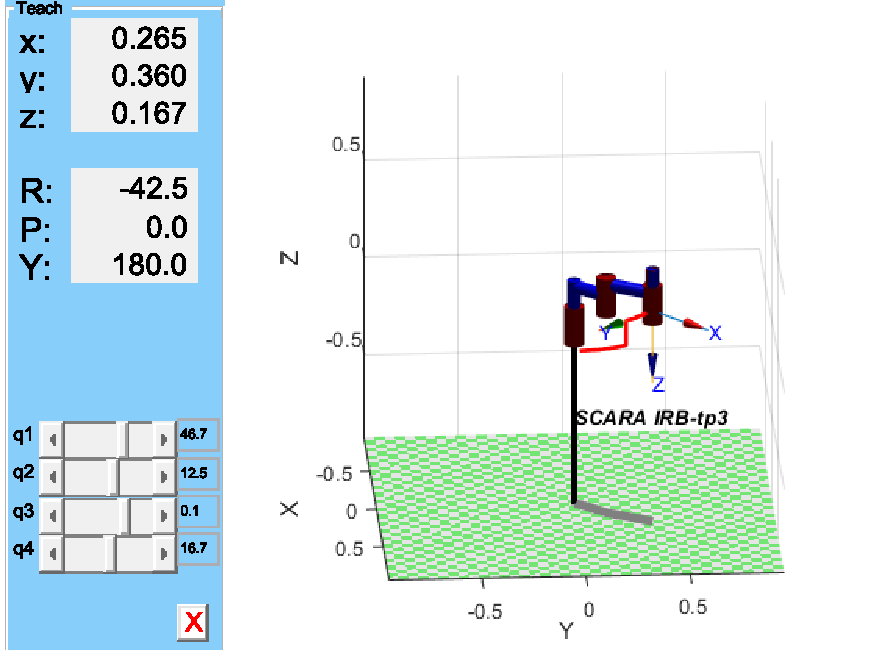
\includegraphics{5-Ejercicio_1_verificacion_Rtp3_teach.pdf}}
    \end{adjustbox}
    \caption{teach Robot tp3}
\end{figure}

\begin{figure}[H]
    \centering
    \begin{adjustbox}{scale = 0.85, max width=\columnwidth}
        \framebox{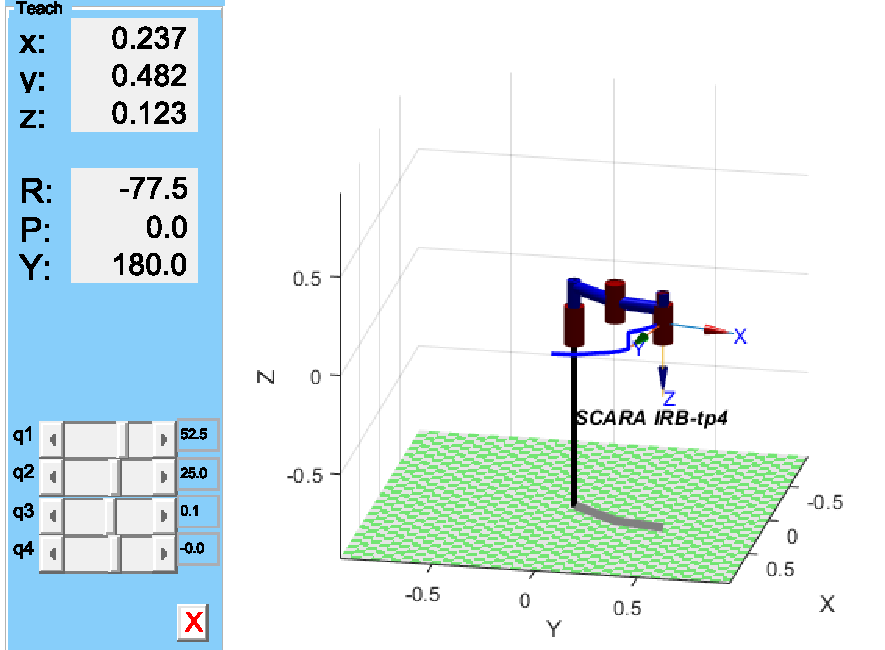
\includegraphics{6-Ejercicio_1_verificacion_Rtp4_teach.pdf}}
    \end{adjustbox}
    \caption{teach Robot tp4}
\end{figure}

\subsection{}
%\begin{equation*}
%    \prescript{O}{}{Rot_M} = 
%    \begin{bmatrix}
%        0.500 & -0.866\\
%        0.866 & 0.500
%    \end{bmatrix}
%\end{equation*}

%\begin{figure}[H]
%    \centering
%    \begin{adjustbox}{scale = 0.85, max width=\columnwidth}
%        \framebox{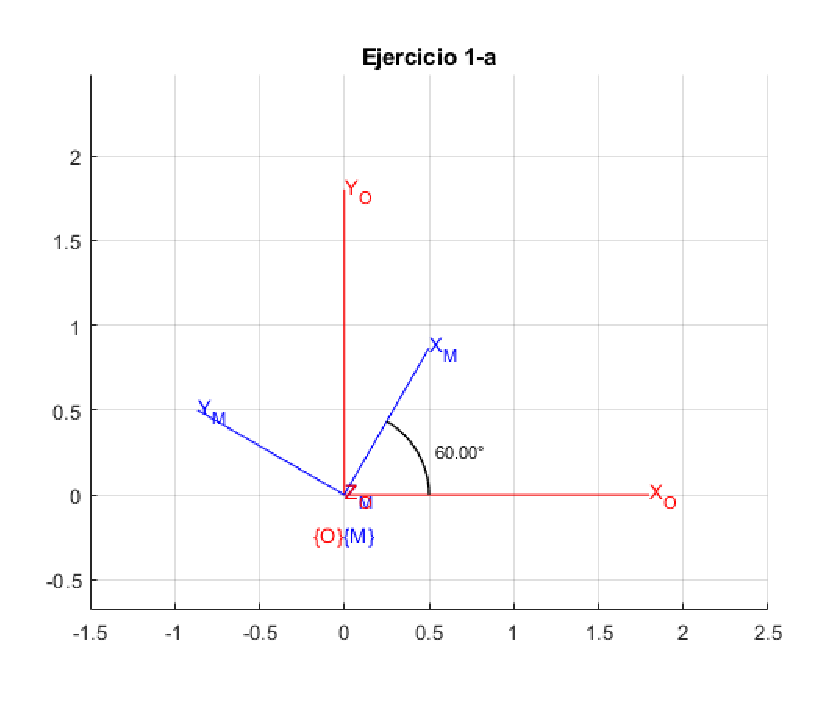
\includegraphics{1-Ejercicio_1_a.pdf}}
%    \end{adjustbox}
%    \caption{Sistema O y Sistema M superpuestos con indicación de ángulo de rotación.}
%\end{figure}


%\begin{table}[H]
%    \centering
%    \begin{tabular}{|c|c|c|c|c|c|}
%    \hline
%    Sistema & $\theta$  & $d$           & $a$    & $\alpha$ & $\sigma$ \\ \hline
%    1       & $q_1$     & $199.2$       & $200$  & 0        & 0        \\ \hline
%    2       & $q_2$     & $59.5$        & $250$  & 0        & 0        \\ \hline
%    3       & $0$       & $q_3$         & $0$    & 180°     & 1        \\ \hline
%    4       & $q_4$     & $37.5$        & $0$    & 0        & 0        \\ \hline
%    \end{tabular}
%    \caption{Parámetros DH alternativos.}
%    \label{parametros DH2}
%\end{table}

\end{document}